\section{Structurally Related Compounds and Transferable Variables}

\begin{figure}[t]
  \centering
  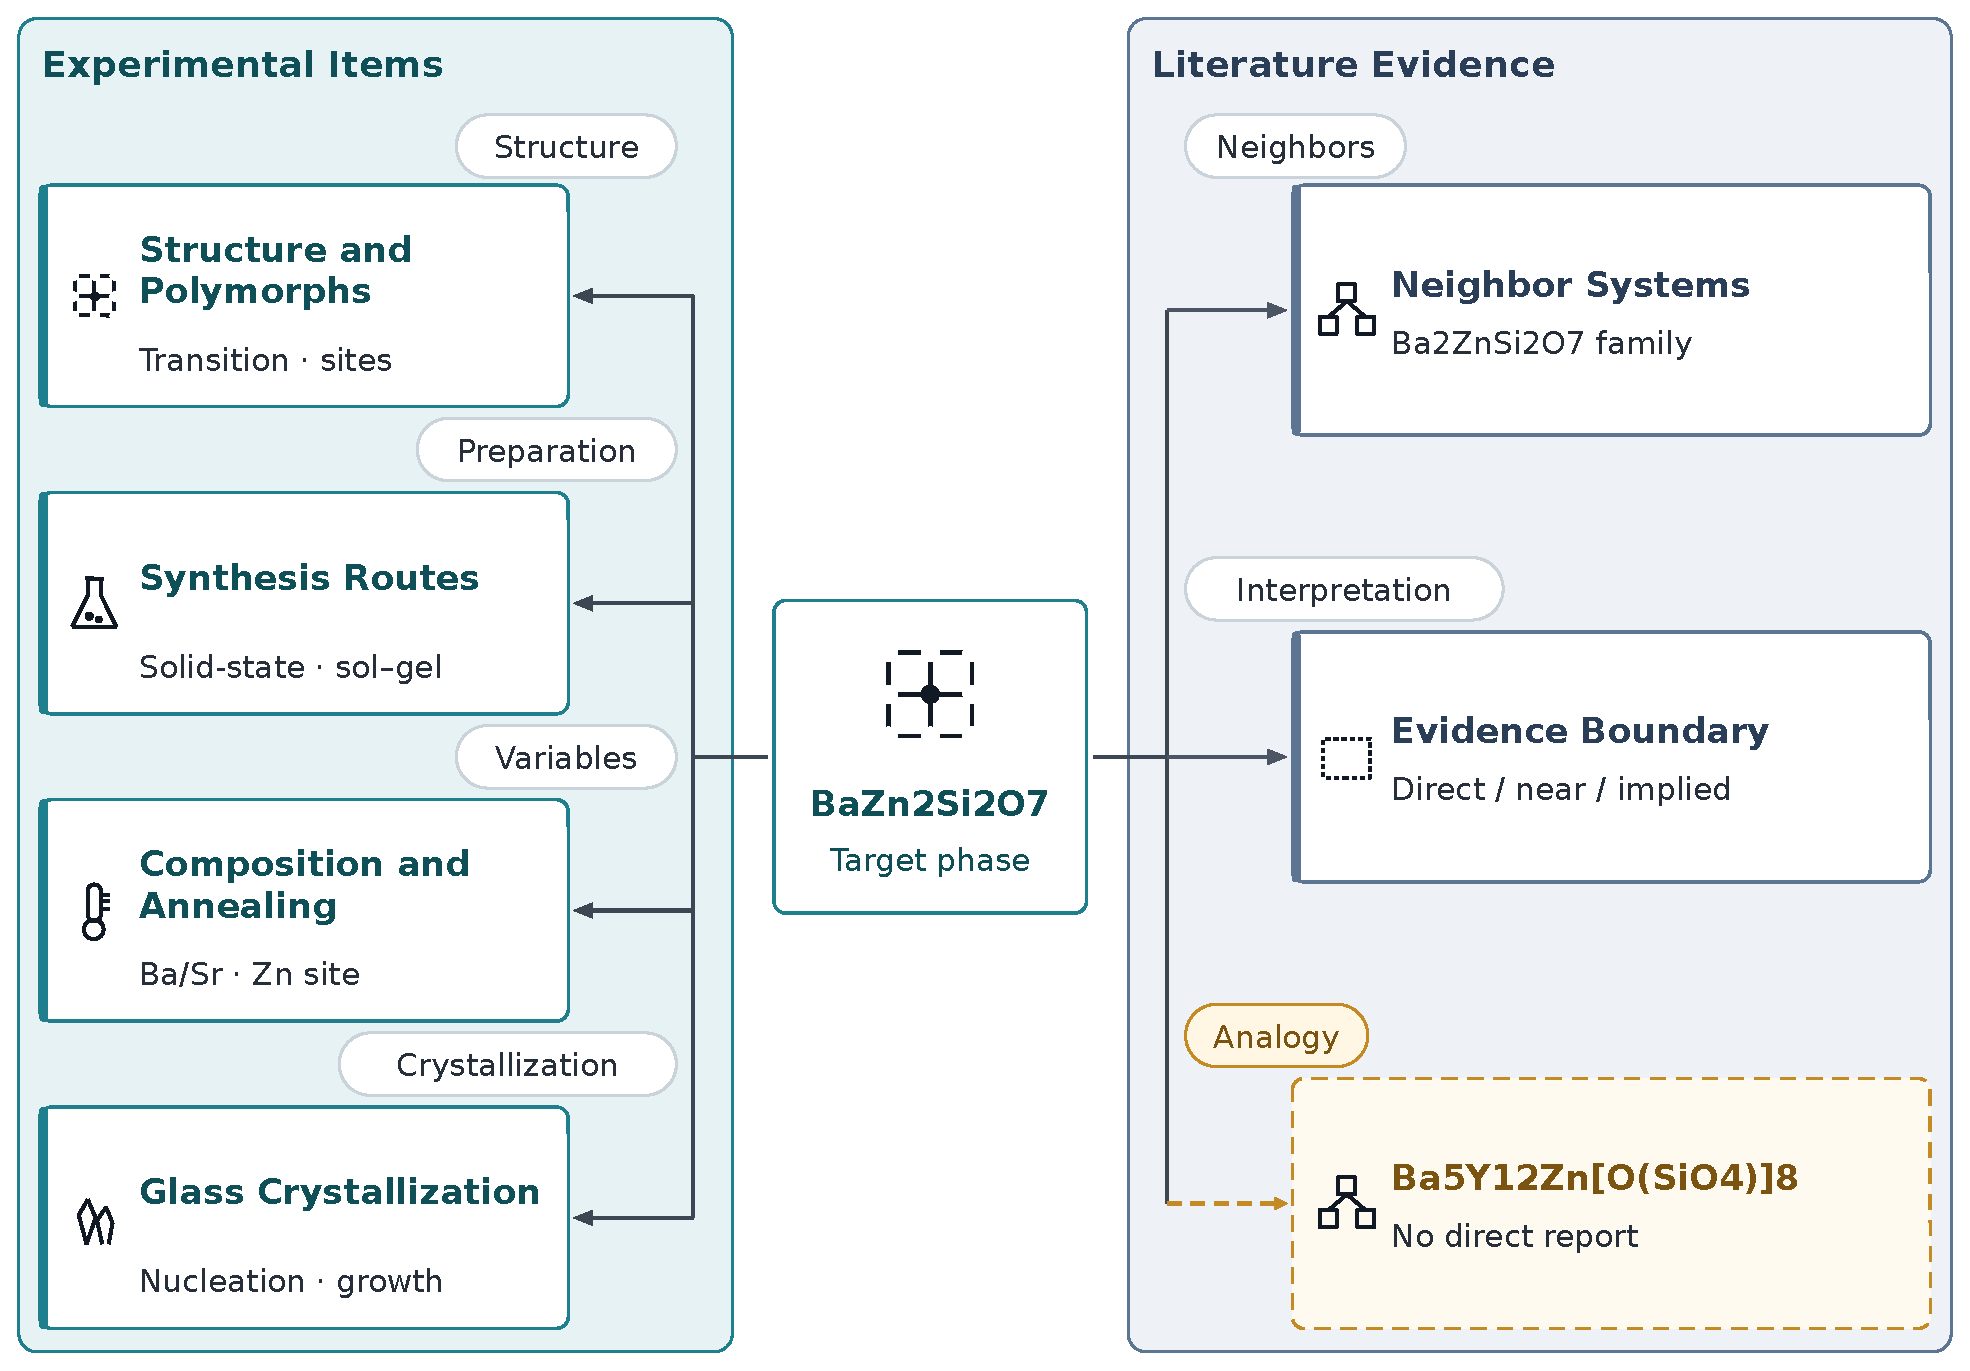
\includegraphics[width=\linewidth]{../figures/pdf/taxonomy_phase_control_en.pdf}
  \caption{\textbf{Taxonomy of BaZn$_2$Si$_2$O$_7$ synthesis and phase control.} Solid branches carry direct experimental evidence for the target phase or experimental evidence from structurally related compounds; dashed nodes mark comparison targets for which no direct structural report exists.}
  \label{fig:taxonomy}
\end{figure}

\subsection{Ba\slash Sr Substitution}

Ba$_{1-x}$Sr$_x$Zn$_2$Si$_2$O$_7$ is the most thoroughly studied isostructural substitution series. Replacing Ba$^{2+}$ with Sr$^{2+}$ lowers the temperature at which the high-temperature phase forms; beyond roughly 10\% substitution the high-temperature structure survives to room temperature and shows near-zero or negative thermal expansion \cite{thieme2015ba1,thieme2016very,thieme2017variable,zou2021near}. Single-crystal XRD identifies this stabilized phase as orthorhombic Cmcm, and the twisting and rocking of the ZnO$_4$ chains is regarded as a major structural origin of the negative thermal expansion \cite{thieme2015ba1}. These results establish A-site cation size and polyhedral voids as effective phase-control variables, but they give no grounds for assuming that Y$^{3+}$ can occupy the same site in large amounts.

\subsection{Zn-Site and Si-Site Substitution}

Divalent cations such as Mg, Co, Mn, Ni, and Cu can substitute for Zn over ranges that differ from one ion to the next. Beyond a critical substitution level the low-temperature structure can reappear, pointing to competition between local coordination preference and long-range phase stability \cite{thieme2016new,kerstan2013bazn2si2o7}. Ge for Si shifts the transition temperature through tetrahedral size and bond flexibility; Ge solubility is limited in Sr-free compositions, whereas Sr-containing compositions retain the high-temperature structure up to higher Ge contents \cite{thieme2016negative}.

\subsection{Glass-Ceramic Processing}

Work on the glass route shows that kinetics matter as much as chemistry. Pt nucleating agents promote heterogeneous nucleation, Nb$_2$O$_5$\slash Ta$_2$O$_5$ change the ratio of surface to bulk crystallization, and noble metals may in addition form alloys or core--shell structures \cite{vladislavova2017heterogeneous,heitmann2019surface,thieme2022noble,thieme2018growth}. Once the grain size falls below about 80~\textmu m, microcracking is reduced and the macroscopic thermal expansion approaches the intrinsic value of the crystal \cite{thieme2016thermal}. Phase-control studies of BaZn$_2$Si$_2$O$_7$ should therefore report phase assemblage, grain size, and crack state together.
